\section {Implementation}
This section describes the technical implementation of the system.
The topic of distribution, parallelism and data handling will be covered.
 Throughout the subsections, fragments of the implementation of two use cases,
  ConnectLobby and TakeTurn, will be provided as examples.

\subsection {Overview}

The overall project solution comprises of a client, server, database and game.
 The client contains the gui and connections to the server. The server hosts
  three services: (1) general service, (2) game service and (3) security token
   service. (1) contains services related to login and account creation. (2)
   contains the services related to lobby connection, matchmaking and taking
    turns. (3) include the services that allow verification and creation of
     tokens to be used with login in (1) and connection in (2).
\\\\
The database itself lies externally to the implementation, but the SQL code
 exists in the solution created from an ADO.NET Entity Model. The game
 includes all the logic and data to create a game locally. This is used
 both for the server and the client to simulate a game. Client and server
  have each their wrapper classes to dictate how the local game is
   controlled and simulated.

\subsection {Distribution}
In this subsection the topic of distribution with focus on a client-server
 environment will be described.

\subsubsection {Communication Protocol}
The communication protocols between server and client are usually either
 Transmission Control Protocol (TCP) or User Datagram Protocol (UDP).
 TCP being a reliable connection-based protocol, whilst UDP is
  not.\footnote{Silberschatz et al. 2010. p. 739} This makes a big
   difference in terms of how the client communicates with the server.
    If a game client is supposed to communicate in real-time with the server,
     then UDP is preferred, as TCP could slow down the messages, or create
      lag over time. If real-time is not necessary, for instance in a simple
       turn-based game, then TCP is preferable, as it ensures messages arrive
        without loss and in the right order. If both are needed, then UDP
        should be chosen, as it can be customized to act as a TCP
         when necessary.

\subsubsection {Connectivity}
Depending on the requirements of the system, the way messages are
handled across computers will be different. Some systems require
multiple servers to distribute computation and management, whilst
others require a simple TCP-connection to a single server.

\subsubsection {Networking Technologies}
In this project, the .NET framework was utilized to both create the
 client and server. The database was created externally. .NET offers
  several technologies to communicate between computers and processes,
   where a few are presented here: (1) Sockets, (2) Protocol listeners
    and clients, (3) Remoting and (4) Windows Communication Foundation (WCF).
\\\\
Sockets allow manual control over inbound and outbound connections, as
 well as what gets sent and received. Sockets, however, operate with bytes,
  which would then require creating a message format to understand the
   message on both the client and server. The protocol listeners and
   clients act as a layer on top of sockets. They present a common interface
    for various protocols to work with, without having to work directly with
    sockets. For instance a TcpListener to create a TCP server.
\\\\
With Remoting a remote proxy marshals calls to a MarshalByRefObject
instance\footnote{Microsoft 1} \footnote{Microsoft 2}. This is reliant
on both client and server having access to the .NET framework. WCF as a
framework has the capabilities of all previous technologies. It uses a
service-oriented architecture (SOA) where services send and receive based
 on requests. This seems similar to Remoting, but WCF allows interoperability
 and integration with industry standards, making it possible to distribute to
  other platforms and framework than .NET.\footnote{Microsoft 3} The
  flexibility of WCF makes it ideal as a choice for networking, which is
  why we have chosen this framework.

\subsubsection {WCF Communication}
In the use case ConnectLobby, the service contract for
IGeneralService (see~\ref{fig:implementation1}) is used to define the
 interface for communication between client and server. The attribute
 ‘ServiceContract’ marks the interface as a contract, whilst the
  ‘OperationContract’ attribute marks a specific entry point in the interface
  for a specific request. The ‘FaultContract’ attribute allows the requests
   to return exceptions of the type ‘FaultException’ if needed.

\begin{figure}[h]
\centerline{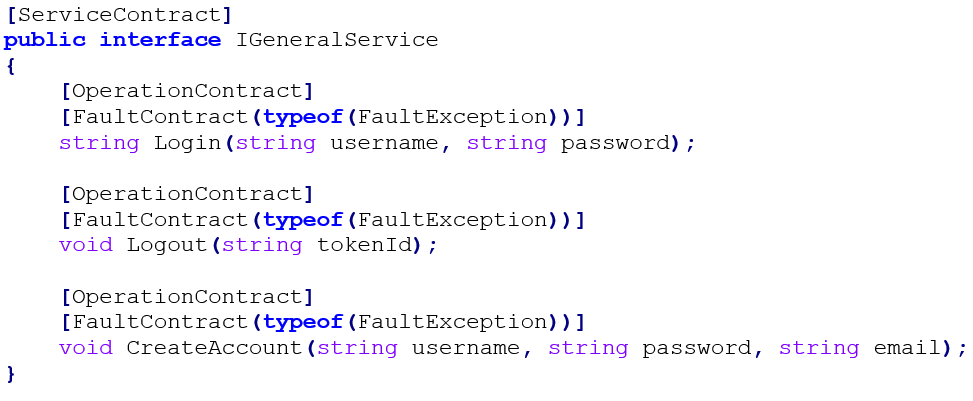
\includegraphics[scale=0.5]{Implementation1}}
\caption {IGeneralService service contract}
\label {fig:implementation1}
\end{figure}

While this settles the client to server messages and return values, it does
 not solve the issue of inter-client communication. Since this project is
  based on the client-server model, the client may not directly message each
   other. Therefore, the server needs to act as a liaison between the clients.
    The two main solutions for this would be a duplex service contract or
    creating client services. Creating a client service would allow easy access
     to all clients, but it would also allow any other person access
      to this service. Ensuring the integrity of the communication could
       prove difficult because of this, as the client service would have
        to verify the messages according to the server’s services.
\\\\
Instead of the client services, we chose the way of a duplex service
contract, which allow two-way communication\footnote {Microsoft 4}. A
duplex service contract requires a specified call-back interface, it is
 here implemented on the client. This allows the server to then send calls
  to the client on demand. The game service is a duplex service
   (see~\ref{fig:implementation2}), allowing the server Lobby to send calls
    to players when certain events occur, like when a turn has been taken.

\begin{figure}[h]
\centerline{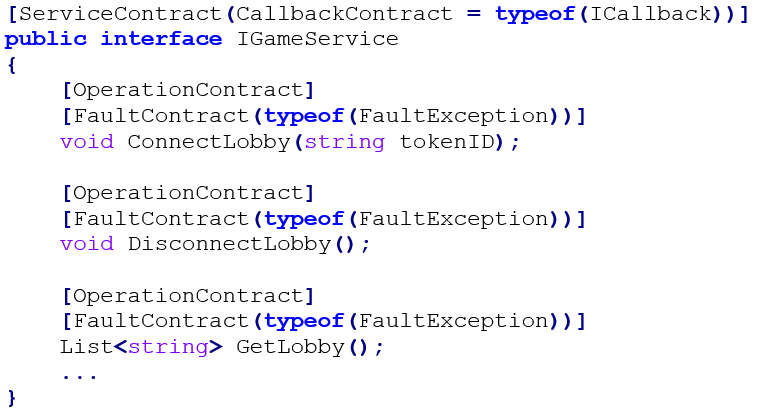
\includegraphics[scale=0.5]{Implementation2}}
\caption {IGameService duplex service contract}
\label {fig:implementation2}
\end{figure}
In order for the client to be able to consume the service, the service
needs to be configured on both ends via the App.config file in each project.
 In the host (here server), a service is configured
  (see~\ref{fig:implementation3}), whilst in the consumer
  (here client) a client is configured.

\begin{figure}[h]
\centerline{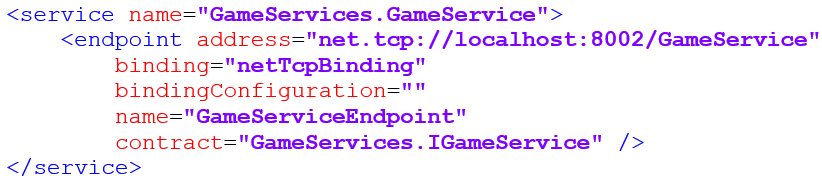
\includegraphics[scale=0.5]{Implementation3}}
\caption {Configuration of IGameService as service}
\label {fig:implementation3}
\end{figure}

After configuration the client can create proxies to the services
 (see~\ref{fig:implementation4}) based on the endpoint specified on the
  server. After creating a channel (proxy), the services can be accessed
   through the contract interface.

\begin{figure}[h]
\centerline{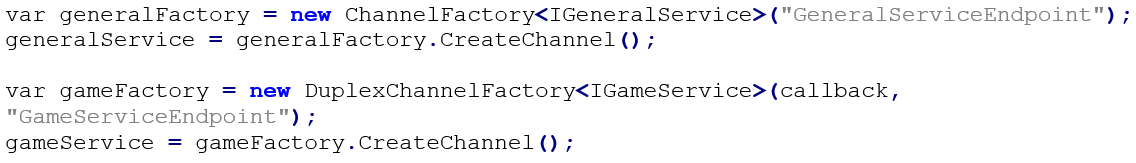
\includegraphics[scale=0.5]{Implementation4}}
\caption {Creating proxies for service access}
\label {fig:implementation4}
\end{figure}

The solution also uses inter-service communication with the security
 token service. The security token service uses a net named pipe binding
  used for on-machine communication, which is used to create and verify
  tokens in the general service and game service.\footnote{Microsoft 5}

\subsubsection {Authentication and tracking}
In order to keep track of the various connections to the game service,
 the IContextChannel - tied to a unique connection - was stored. This
 would then also be used to verify incoming requests to avoid requests
 that could change the internal state of the server game and lobby
  unexpectedly. The channel would also be needed in order to get the
   matching call-back connection to the client.

\subsection {Parallelism}
In this subsection the topic of parallelism with focus on threading and
concurrency will be described.

\subsubsection {Threading}
The major concerns in terms of threading is avoiding freezing up the GUI
by calling services, which may or may not have a considerable delay with
 its return. Therefore, all calls to the services are threaded using
 ThreadPool.QueueUserWorkItem (see~\ref{fig:implementation5}), which
 will invoke a delegate in its own thread. This thread is managed in
 the background, removing it if all foreground threads
  terminate.\footnote{Microsoft 6}

\begin{figure}[h]
\centerline{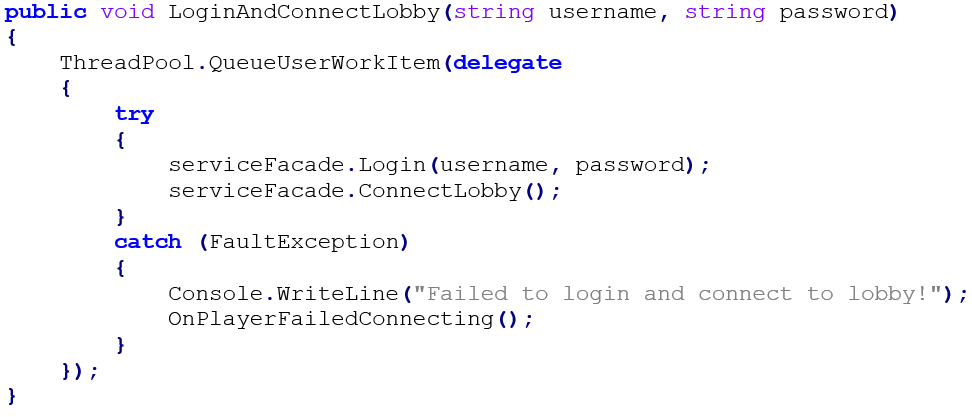
\includegraphics[scale=0.5]{Implementation5}}
\caption {Queuing the ThreadPool}
\label {fig:implementation5}
\end{figure}

When call-backs are made to the client, the client invokes events.
 These events are observed by GUIFacade. Here the GUIFacade is
  supposed to change the GUI based on the type of event. To ensure
   being able to access the UI thread in WPF, a Dispatcher is used.
    The Dispatcher is a service manager for providing work to a single
     thread. For every event the Dispatcher is invoked
     (see~\ref{fig:implementation6}), which allows the events invocations
      to continue without waiting for the GUI update.\footnote{Microsoft 7}

\begin{figure}[h]
\centerline{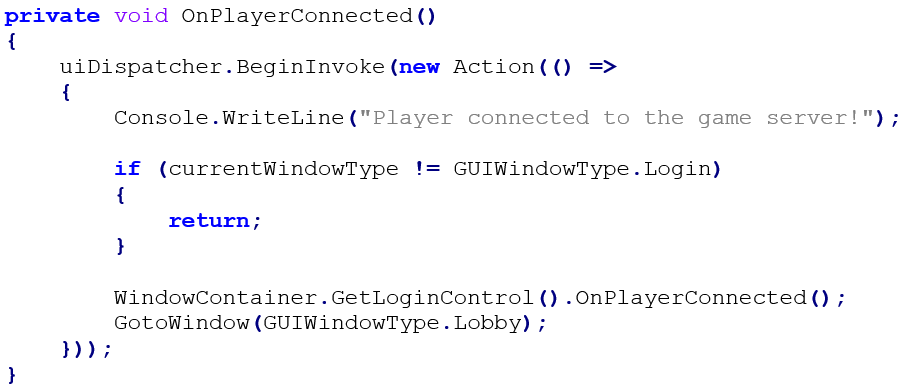
\includegraphics[scale=0.5]{Implementation6}}
\caption {Invoking the UI dispatcherl}
\label {fig:implementation6}
\end{figure}

\subsubsection {Concurrency}
As any number of clients could potentially connect to the services, the
service is required to be thread-safe to ensure a stable internal state.
WCF by default marks services as having a concurrency mode of ‘Single’,
 automatically making the service instances thread-safe. This is done by
  only allowing one call to enter at a time, each waiting to acquire the
  synchronization lock. If the calls are unable to get the lock, they will
   wait in an ordered queue.\footnote{Microsoft 8}
\\\\
This heavily limits the service in terms of requests handled over time. For
 the current state of the project, this is not a problem, as only a few
  clients are connected, and they send out requests infrequently. If the
  project needed to be up scaled, however, the concurrency mode of the
  service would need to be set to ‘Multiple’, effectively removing the
  automatic thread-safety. The concurrently accessed data would then
   need to be synchronized manually.\footnote{Microsoft 8}
\\\\
The last concurrency mode is ‘Reentrant’. It is a variant of the ‘Single’
 mode, also thread-safe, allowing call reentrancy. This means that a call
 is allowed to be called again in the same context used to enter the first
 time. This avoids potential deadlocks for something like call-backs, where
  a call-back method may call the same service call that caused the call-back
   method to be called.\footnote{Microsoft 8} This mode is set on the game
   duplex call-back in the client to avoid problems with calls reentering.
   Currently, though, the effects of this is not noticed, as the GUI threads
    the called events.
\\\\
While the service itself is thread-safe, the resources it accesses are not by
 default. Although, in our implementation only one service accesses the
 resources supplied in its own project. Since only one call is allowed at a
  time per service, the resources inside should be safe. The only resource
  in the client that would need synchronization is the token ID string, but
   since strings are immutable it should already be thread-safe, as the
    internal state doesn’t change.

\subsection {Data Handling}
In this subsection the topic of data handling with focus on serialized
objects, data protection and the database will be described.

\subsubsection {Serialized Objects}
All primitive and most common types are automatically supported for
serialization in WCF when they are used for return values or
arguments\footnote{Microsoft 9}. In order to serialize custom data
structures, however, a data contract must be defined, so that both
the host (service) and consumer (client) understands the interface
language.\footnote{Microsoft 10}

\textbf {Data Transfer Object (DTO)}
The data contracts (see~\ref{fig:implementation7}) act as data
transfer objects, serving the purpose of sending data without behaviour
 or logic. They are defined by the ‘DataContract’ attribute and
  ‘DataMember’ attribute.

\begin{figure}[h]
\centerline{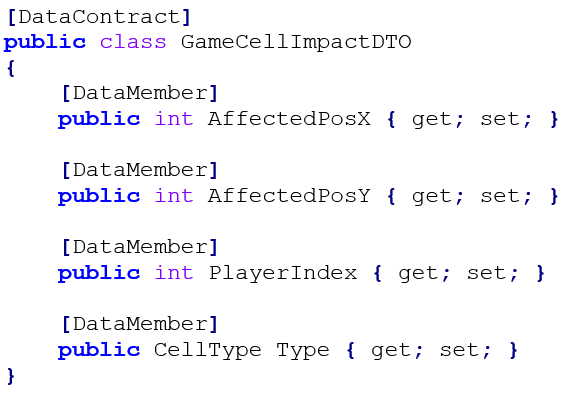
\includegraphics[scale=0.5]{Implementation7}}
\caption {DataContract for cell impact callbacks}
\label {fig:implementation7}
\end{figure}

\subsubsection {Data Protection}
Protecting data comes in various degrees, where some are more
vulnerable than others if accessed by the wrong people or processes.
 In order to ensure secure transmission of data, two major areas
  need to be considered:
\begin{enumerate}
	\item Communication channel
	\item Data storage
\end{enumerate}

\textbf {Sensitive Data}
Sensitive data, such as credentials, send through the communication
 channel between client and server needs to be handled sensitively.
  Sending credentials as plain text will allow anyone listening to
  the channel to fetch the data. This would allow the listener to
  spoof or imitate a user, or in the worst case allow access to
   other sensitive user information.
\\\\
Securing data transfer in WCF can be done by using transport
security or message security. Transport security is ideal for
 intranets, whilst message security is ideal for internets.
  This is an area in which the group did not spent a lot of time in.
   This also means that credentials aren’t protected currently,
    but they would be a priority for future iterations.\footnote{Microsoft 11}
\\\\
Using a technology such as SSL or TLS will provide message integrity
 and message confidentiality. Message integrity ensures that the messages
 are not modified while transferring. Message confidentiality ensures
  that the messages stay privately known while
  transferring.\footnote{Microsoft 12}

\textbf {Tokens}
Once a secure channel has been created, the user can send their
credentials to the target server. The login server then responds
 by providing the user with a token from the security token service.
 The server can use token-based authentication for all future requests
 for that specific user. This is done by creating a security token that
 is returned to the user. The user then sends this token to the server for
  initial requests to services using this login system to verify the user
   and lock the token in place.

\textbf {Database}
The database was created using ADO.NET Entity Model, which can create a
ready-to-go database based on the entity model. Using the entity model
 makes it easy to add new data in the database or extract
  information (See~\ref{fig:implementation8}).

\begin{figure}[h]
\centerline{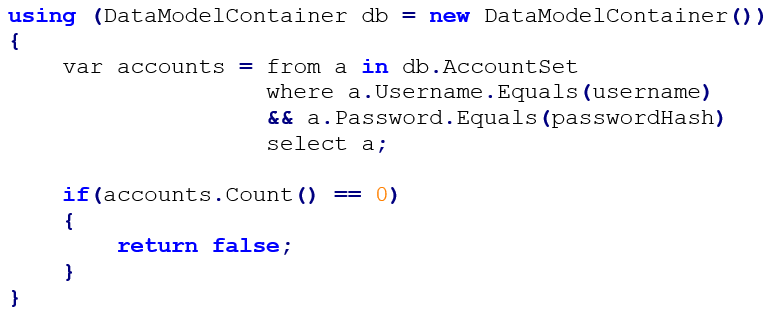
\includegraphics[scale=0.5]{Implementation8}}
\caption {Using entity model container}
\label {fig:implementation8}
\end{figure}

As of now only user accounts are stored in the database
(see~\ref{fig:implementation9}), since multiplayer games need to be
 finished in one session. New accounts are created through the general
  service, contacting the entity model.

\begin{figure}[h]
\centerline{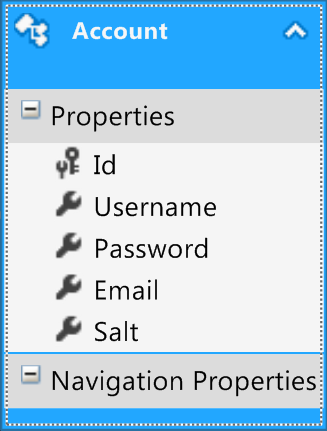
\includegraphics[scale=0.35]{Implementation9}}
\caption {Account entity}
\label {fig:implementation9}
\end{figure}

\textbf {Hashing and Salting}
Storing sensitive data as plain text in the database would allow
anyone with access to the database to read and potentially exploit
each entry. Therefore all passwords get hashed with a
salt (see~\ref{fig:implementation10}), where both the hashed password with
 salt and the salt itself is stored in the database. The username and email
  are not hashed for the database, as they are needed for quick look-up in
   the database, so that the salt can be retrieved to check the password.
    The username is however hashed with a salt for the token that needs to
     be returned.

\begin{figure}[h]
\centerline{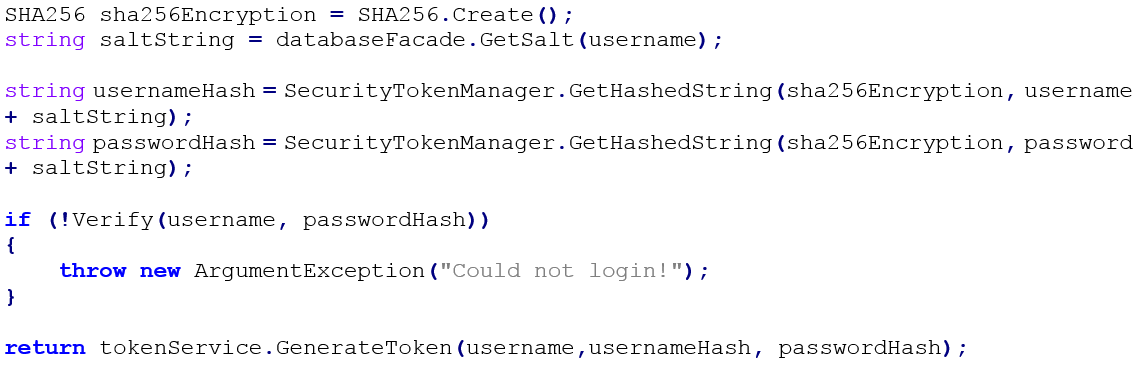
\includegraphics[scale=0.5]{Implementation10}}
\caption {Hashed salt of password}
\label {fig:implementation10}
\end{figure}
